\chapter{系统拓扑结构研究}
\label{cha:SystemTopology}

经过第\ref{chapter:Introduction}章的分析,本文确立了研究目标和研究内容,其中梯级系统拓扑结构的选择是直接关系到梯级系统能否安全高效运行的先决条件,一个具有不合理拓扑结构的梯级系统甚至不能正常运行。梯级系统以现有成熟光热发电技术为基础,经过对梯级太阳能光热发电的多种影响因素的分析和排除,选择应用于梯级系统的各部件,经过合理的布局,确定有效的梯级太阳能光热发电的拓扑结构方案。

现有的经过商业验证的太阳能热发电技术有三种——太阳能槽式发电,太阳能碟式发电和太阳能塔式发电。
由于太阳能塔式发电系统占地面积较大,投资成本太高,考虑到未来需要搭建太阳能光热梯级发电示范系统,本文仅选择两种太阳能光热发电技术(太阳能槽式发电和太阳能碟式发电)作为太阳能光热梯级发电系统设计的基本系统。为了实现对太阳能碟式集热器获得的高温热量进行梯级利用,采用空气(或氮气)作为太阳能碟式发电系统的传热介质来传输所收集的热量。
\begin{figure}[!ht]
\centering
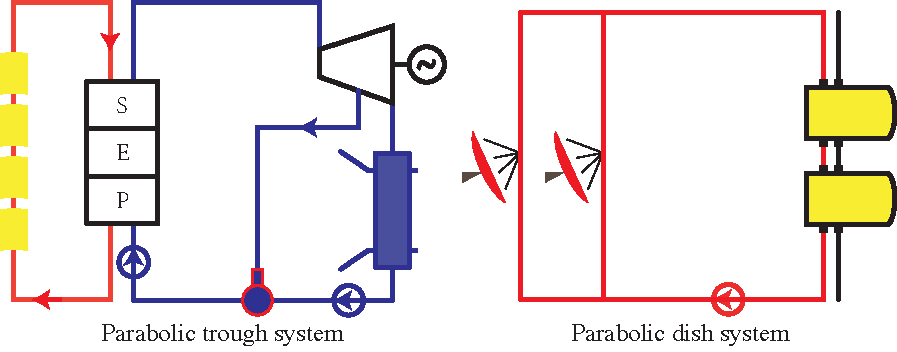
\includegraphics[width=0.8\textwidth]{fig/PTPD.pdf}
\caption{太阳能槽式发电系统和太阳能碟式发电系统结构示意图}
\label{fig:PTPD}
\end{figure}
典型的太阳能槽式发电系统和太阳能碟式发电系统的结构示意图如图\ref{fig:PTPD}所示。为使本文中的系统结构图更加清晰一致,图\ref{fig:Legends}列出了太阳能光热发电系统中可能出现的所有元件的图例。
\begin{figure}[!ht]
\centering
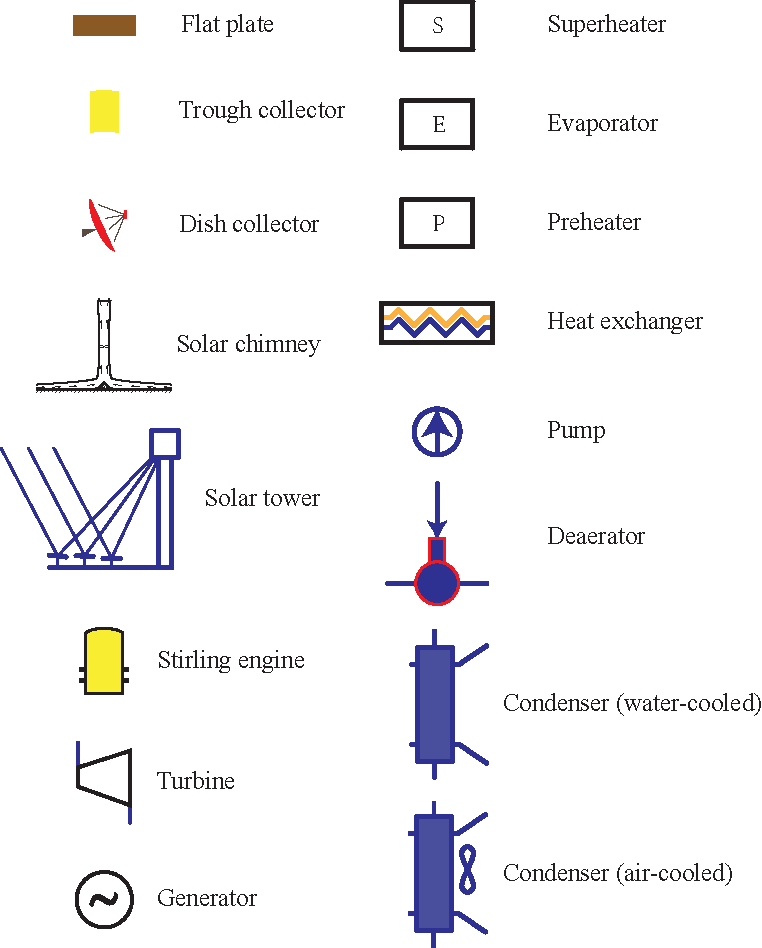
\includegraphics[width=0.65\textwidth]{fig/Legends.pdf}
\caption{太阳能光热发电系统中的元件列表}
\label{fig:Legends}
\end{figure}

利用这两种基本系统,通过选择不同的系统拓扑结构,来实现能量的梯级收集和梯级利用。由于梯级系统的拓扑结构需要考虑多种因素,例如水工质朗肯循环或有机工质朗肯循环、多种集热器的配合使用、不同热力循环的组合等,梯级系统可以组合的拓扑结构的数量非常之多。为了获得最合适的梯级系统拓扑结构,需要从可行性、经济性等角度仔细分析这些因素。需要说明的是,本文进行的研究没有考虑采用蓄热系统,这是因为:(1) 本文重点在于从理论上分析梯级系统能量的梯级收集和梯级利用,分析的条件是基于系统稳态运行的假设,所以无需设置蓄热器。(2) 蓄热器的存在将会改变系统的集热温度和供热温度的匹配性,给系统的分析带来额外的工作量。(3) 本文拟建立的梯级示范系统仅用于实验研究,暂不考虑将发出的电能并网,而蓄热系统的加入会产生额外的成本。(4) 蓄热系统可以在后续研究工作中引入,而不影响本文的研究内容和结论。

\section{基于朗肯循环的系统结构}
\label{sec:RankineCycleBased}

朗肯循环的系统结构主要受朗肯循环工质的影响,水工质朗肯循环(SRC)太阳能光热系统的典型结构示意图和有机工质朗肯循环(ORC)太阳能光热系统的典型结构示意图分别如图\ref{fig:TypicalSteamRankineSolarSystem}和图\ref{fig:TypicalOrganicRankineSolarSystem}
所示。本节主要研究朗肯循环工质的选择问题。

\noindent \begin{figure}[htbp]
\centering
	\begin{subfigure}[b]{0.4\columnwidth}
	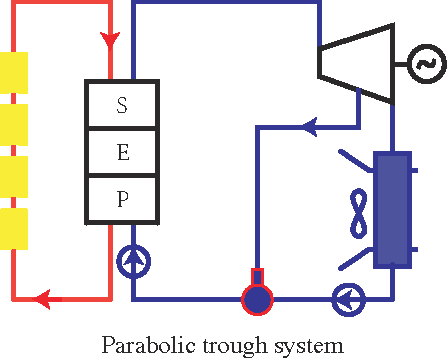
\includegraphics[width = \columnwidth]{fig/TypicalSteamRankineSolarSystem}
	\caption{}\label{fig:TypicalSteamRankineSolarSystem}
	\end{subfigure}
	~
\begin{subfigure}[b]{0.4\columnwidth}
	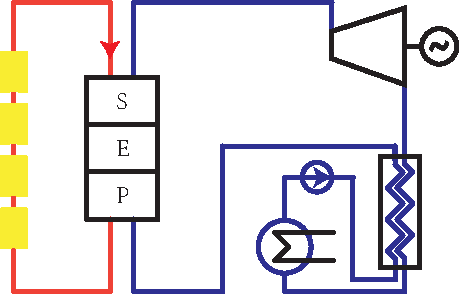
\includegraphics[width = \columnwidth]{fig/TypicalOrganicRankineSolarSystem}
	\caption{}\label{fig:TypicalOrganicRankineSolarSystem}
	\end{subfigure}
	\caption{采用SRC和ORC的太阳能光热系统的典型结构示意图}
	\label{fig:TwoTypesOfRankineCycle}
\end{figure}


\subsection{理想朗肯循环工质特点}
\label{sec:IdealRankineCycleFluid}

\begin{figure}[!ht]
\centering 
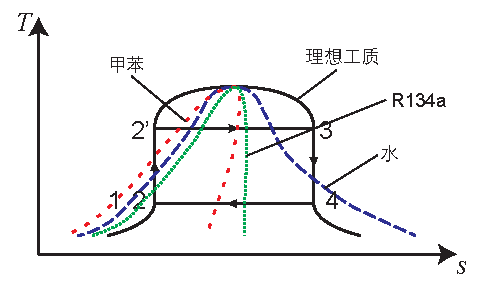
\includegraphics[width=0.5\textwidth]{fig/idealTs}
\caption{用于朗肯循环的理想工质的温熵图}
\label{fig:idealTs}
\end{figure}

应用于朗肯循环的不同工质的温熵曲线如图\ref{fig:idealTs}所示。需要说明的是,图中各曲线只是用于表示不同工质的饱和曲线形状,曲线对应的熵值和温度不代表其真实熵值和温度,也不能用于不同工质之间的比较。其中,理想工质具有以下特点\cite{Abbin1977}:
\begin{itemize}

	\item 饱和液体的比热容要小,这样图\ref{fig:idealTs}中的曲线2-2'才接近竖直。
	\item 临界点温度要高于最高运行温度,以使所有的吸热过程都发生在临界点温度以下。
	\item 最高运行温度所对应的饱和蒸汽压力应该适中,以便安全运行并有利于降低设备的制造成本。
	\item 凝气温度下对应的蒸气压力应该高于大气压,以避免空气泄漏到系统中。
	\item 状态点4的蒸气的密度应该较大,这样可以避免大尺寸的汽轮机叶片,壳体和换热器。
	\item 图\ref{fig:idealTs}中气态饱和曲线3-4应该接近竖直,从而避免汽轮机中的工质膨胀进入湿蒸汽区($ds/dT < 0$的情况)或是过热区($ds/dT > 0$的情况)。
	\item 对于小功率汽轮机的应用,工质应该具有较高的分子量以便于减小汽轮机的转速和(或)减少级的数量,并且允许合适的质量流量和汽轮机喷嘴面积。
	\item 工质在常温常压下为液体,以便于运输和控制。
	\item 工质的凝固点应该低于工作的环境温度。
	\item 工质具有良好的传热性能,价格便宜,在最高操作温度下热稳定较好,不易燃烧,无腐蚀性,无毒性等。
\end{itemize}

\subsection{水工质朗肯循环和有机工质朗肯循环的特点}
\label{sec:RankineCycleFluid}

水是朗肯循环中最常用的工质,水工质朗肯循环的各部件相关的技术比其他工质更为成熟。水的价格便宜(虽然锅炉级的水必须是高度蒸馏的,因此成本比自来水高),水工质朗肯循环的高压部分的密封并没有其它工质那么重要。此外,蒸汽的不易燃性和可用性是其额外的优点。因为它的临界温度和压力分别为374$\mathrm{^\circ C}$和22$\,\mathrm{MPa}$,它可以在中等压力下实现较高温度的等温吸热。

水工质朗肯循环也存在一些缺点。蒸汽的低温特性并不理想,因为蒸汽在常温下具有很低的蒸气压和密度(参见表\ref{tab:waterT_P_D})。对于低压部件,保持密封性,防止空气泄漏是设计中需要注意的问题。
\begin{table}[htbp]
\setlength{\abovecaptionskip}{-10pt}
	\caption{不同温度下饱和蒸汽的压力和密度}
	\begin{center}
	\begin{tabular}{cccccccccc}
		\toprule	
		    $T$(K)    &	373.15	    &    363.15    &    353.15    &    343.15    &    333.15    &    323.15    &    313.15    &    303.15    &    293.15\\
		\midrule	
		    $p$(Pa)    &    101322        &    70117    &    47373    &    31176    &    19932    &    12344    &    7381    &    4246    &    2339\\
		    $\rho$($\mathrm{kg/m^3}$)    &    0.5982        &    0.4239    &    0.2937    &    0.1984    &    0.1304    &    0.0831    &    0.0512    &    0.0304    &    0.0173\\
		\bottomrule
	\end{tabular}
	\end{center}
	\label{tab:waterT_P_D}
\end{table}

%The organic Rankine cycle can be used in the solar parabolic trough technology in place of the usual steam Rankine cycle. The ORC allows power generation at lower capacities and with a lower collector temperature, and hence the possibility for low-cost, small scale decentralized CSP units. Most organic fluids used in organic Rankine cycle are drying fluids. The vapor leaving the expander still contains heat that can be transferred to the compressed liquid stream because the turbine outlet temperature is above the condenser temperature. A vapor-to-liquid heat exchanger, known as a regenerator, is typically used for this purpose.
%Figure~\ref{fig:TypicalOrganicRankineSolarSystem} shows the schematic diagram of a typical organic Rankine cycle solar system.
有机工质朗肯循环也可应用于太阳能槽式发电,取代常见的水工质朗肯循环。ORC可以在小功率和低集热温度的条件下进行发电,因此可以用于生产低成本,小规模的分布式CSP装置。ORC中使用的大多数有机工质是干流体(温熵图上$ds/dT > 0$)。汽轮机出口的气体具有一定的过热度,由于汽轮机出口温度高于冷凝器温度,所以可以将一部分热量传递给压缩过的液态有机工质。回热器就是为了回收利用这一部分热量而设计的,回热器为过热蒸气-过冷液体换热器。
%典型的有机工质太阳能光热系统结构示意图如图\ref{fig:TypicalOrganicRankineSolarSystem}所示。

%Compared with steam for the Rankine cycle, it has the following advantages:
与水工质朗肯循环相比,它具有以下优点:
\begin{itemize}
%  \item  Small turbine head allows for moderate shaft speed and a single- or two-stage design.
	\item 在中等转速和单级或双级的设计条件下可以实现小型汽轮机应用。
%    \item Low volume ratio facilitates the flow path design.
    \item 较低的体积比更有利于流道的设计。
%    \item High volume flow and low velocity of sound results in reasonable flow areas.
    \item 较高的体积流量和音速值便于设计合理大小的通流面积。
%    \item Low temperature drop during expansion reduces thermal stress problems.
    \item 有机工质在膨胀的过程中温降很小,这有利于减少热应力导致的各种问题。
%    \item Dry expansion avoids blade erosion caused by vapor wetness.
	\item 干流体可以避免由于乏气存在湿度造成的叶片侵蚀。
%    \item Low system pressure facilitates housing design.
	\item 较低的系统运行压力便于一体化设计。
  \end{itemize}
  
\subsection{朗肯循环工质的选择}
\begin{figure}[!ht]
\centering 
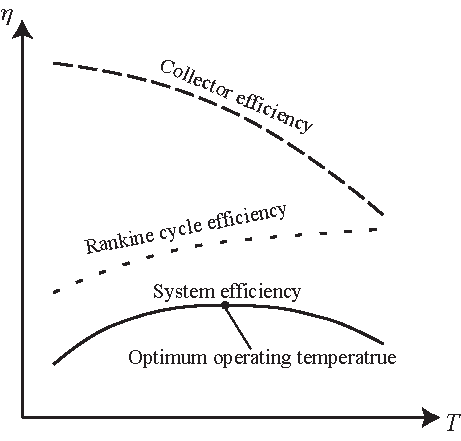
\includegraphics[width=0.5\textwidth]{fig/Efficiency}
\caption{不同运行温度下的效率曲线}\label{fig:Efficiency}
\end{figure}
选择朗肯循环太阳能系统的工作流体时需要考虑两个重要方面:
\begin{enumerate}
  \item 选择的工作流体易于在最佳运行温度条件下运行。
 对于朗肯循环太阳能光热系统,集热器效率随着工作温度的升高而降低,朗肯循环的效率随着工作温度的升高而升高,系统的总效率存在如图\ref{fig:Efficiency}所示的最佳工作温度。工作流体应当有利于达到该最佳工作温度。    
  \item 如果使用传热流体,则传热流体的状态需要和热力循环的工作流体的状态相匹配。
  一方面,工作流体的工作温度应该低于传热流体的收集温度。另一方面,工作流体的工作温度不应该比传热流体的收集温度低很多,以避免换热过程中产生大量的㶲损失。
\end{enumerate}

第\ref{sec:RankineCycleFluid}节中详细介绍了水和有机工质作为朗肯循环的工作流体所带来的优缺点。很清楚,对于低参数和小容量的配电发电,有机工质将是更好的选择,否则水是更好的选择。鲍军江和赵力\cite{Bao2013}对工作流体的选择(包括纯液体和混合液)进行了全面的综述。在该综述中,考虑了许多因素,如操作条件,工作流体的特性,设备结构和环境安全等。
必须指出的是,工作流体的种类(主要是干流体或湿流体)会影响系统的运行和布局。

\section{槽式朗肯循环与太阳能烟囱技术集成的系统结构}
\label{sec:sc}

太阳能烟囱电站也被称为太阳能气流电站,直接(不聚光)利用太阳产生的热能来发电。太阳能烟囱发电系统由太阳能集热棚、太阳能烟囱和涡轮机发电机组3个基本部分构成,典型的太阳能烟囱电站的示意图如图\ref{fig:SolarChimney}所示。太阳能烟囱电站建立在太阳辐射强度高,土地保温性能好的地区。集热棚离地面有一定距离,其外围周边是开放的。太阳能烟囱和集热棚连接,位于集热棚中央。涡轮机发电机组位于烟囱底部。
在这种电站中,空气在半透明的集热棚下因温室效应而升温。集热棚的周边是开放的,外部空气由于密度分布不同而流入集热棚,然后在浮力的作用下热空气流入烟囱产生热气流。在气流的路径上设置有涡轮机发电机组,用于将气流的动能转化为电能。

\begin{figure}[!ht]
\centering 
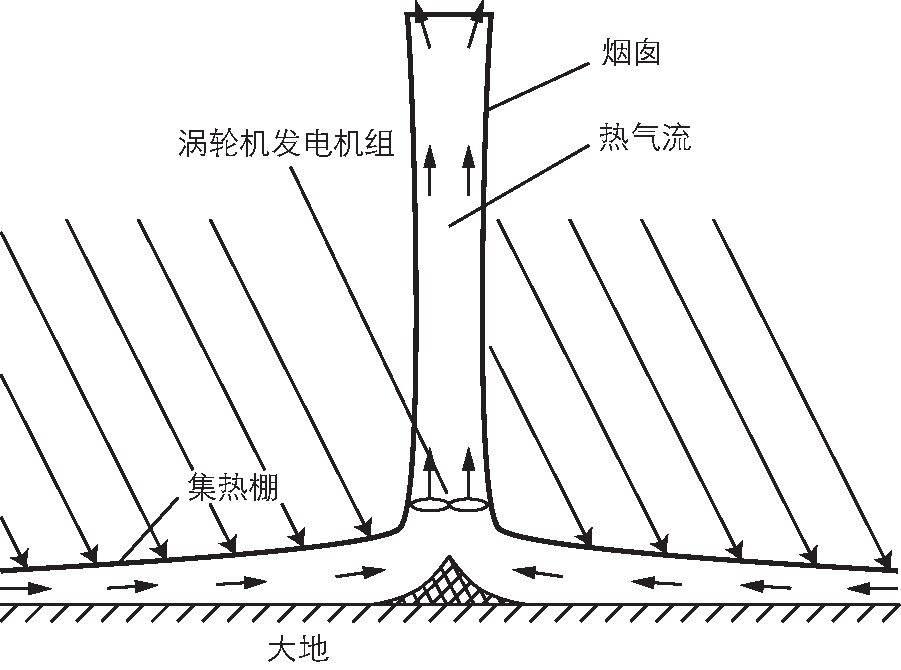
\includegraphics[width=0.5\textwidth]{fig/SolarChimney}
\caption{太阳能烟囱电站的结构示意图}\label{fig:SolarChimney}
\end{figure}

太阳能烟囱可以利用低温热源(低品位能源)发电。因此,槽式系统和太阳能烟囱的组合可以作为能源梯级利用的有效途径。在组合系统中,朗肯循环中的冷凝器采用空冷。空冷风扇将冷却过冷凝器的热空气从太阳能烟囱的周边吹入太阳能烟囱发电厂。热气流汇聚在烟囱底部,在浮力作用下向上流动,带动烟囱内的涡轮机发电机组,从而实现朗肯循环凝结热的有效利用。
图\ref{fig:CombinedSolarChimney}显示了一个槽式系统和太阳能烟囱组合的例子。

\begin{figure}[!ht]
\centering 
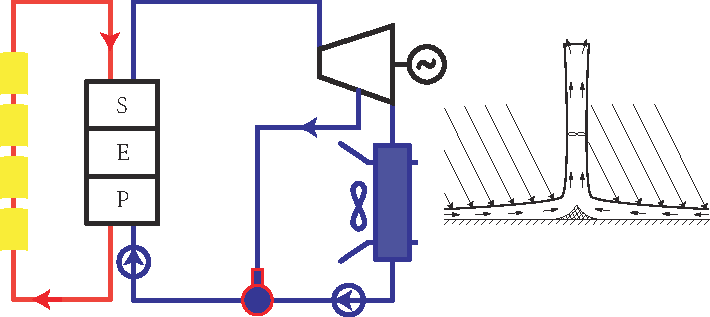
\includegraphics[width=0.7\textwidth]{fig/CombinedSolarChimney}
\caption{槽式系统和太阳能烟囱组合结构示意图}\label{fig:CombinedSolarChimney}
\end{figure}
然而,目前的太阳能烟囱系统的效率非常低。Bilgen和Rheault利用MATLAB建立了5$\,\mathrm{MW}$的太阳能烟囱模型\cite{Bilgen2005}。他们对不同地理位置,不同烟囱高度和集热器高度的太阳能烟囱电站进行了模拟分析。其主要设计数据及计算结果如表\ref{tab:sc}所示。 初步的设计参数为太阳辐射强度为1000$\,\mathrm{W/m^2}$,额定功率为5$\,\mathrm{MW}$。从表中可以发现,烟囱效率和系统总效率都很低,太阳能烟囱技术仍处于初步发展阶段。
\begin{table}[htbp]
\setlength{\abovecaptionskip}{-10pt}
	\caption{太阳能烟囱设计参数及模拟结果}
	\begin{center}
	\begin{tabular}{ccccc}
		\toprule
		地理位置	&Ottawa    &Winnipeg    &Edmonton    &Schlaich\\
		\midrule
		集热棚直径 (m)    &	1110	&	1110	&	1110	&	1110 \\
  集热棚面积 ($\mathrm{m^2}$)    & 950000    & 950000	&	950000	&	950000\\
  烟囱高度 (m)    &123    &60    &    35&    547\\
  集热器高度 (m)    &848    &975    &1024    &    -\\
  烟囱直径 (m)    &54    &54    &54    &54\\
  集热棚内温升 ($\mathrm{^\circ C}$)    &25.9    &25.9    &25.9    &25.9\\
  气流速度 (m/s)&9.1    &9.1    &9.1    &9.1\\
  总压头 (Pa)&518.3    &518.3    &518.3    &383.3\\
  平均效率\\
  集热棚 (\%)    &56.00    &56.00    &56.00    &56.24\\
  烟囱 (\%)    &1.82    &1.82    &1.82    &1.45\\
  涡轮机 (\%)    &77.0    &77.0    &77.0    &77.0\\
  系统整体 (\%)    &0.79    &0.79    &0.79    &0.63\\
		\bottomrule
	\end{tabular}
	\end{center}
	\label{tab:sc}
\end{table}
 
另外,太阳能烟囱成本高,占地面积大,不利于今后搭建太阳能光热梯级发电示范系统。鉴于这些,梯级系统不采用太阳能烟囱技术。

\section{多种集热方式集成的系统结构}
\label{sec:csc}
考虑到每种类型的集热器都有其适宜的工作温度范围,集成使用多种集热方式,采用多种集热器逐步加热传热流体是实现梯级集热的可行方案。
槽式集热器和菲涅耳集热器更适合于低温集热,碟式集热器和塔式集热器更适合于高温集热。串联连接不同类型的集热器可以有效利用它们各自的优点。图\ref{fig:SeriesCollector}给出了一个采用集热器串联连接的梯级系统的方案。在这个系统中,空气作为传热介质在流入碟式集热器之前先被槽式集热器预热。槽式集热器用于收集低温热能,碟式集热器用于收集高温热能。

\begin{figure}[!ht]
\centering 
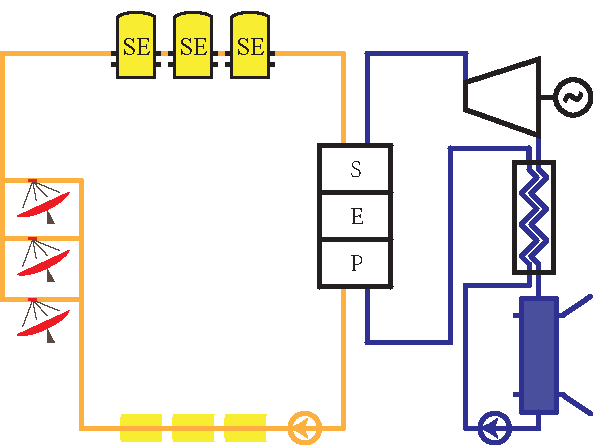
\includegraphics[width=0.5\textwidth]{fig/SeriesCollector}
\caption{一种采用集热器串联连接的梯级系统方案}\label{fig:SeriesCollector}
\end{figure}

在这种方案中,空气依次在槽式集热器和碟式集热器中被加热。为斯特林机提供热量后,热空气流入换热器为朗肯循环提供热量。在这种拓扑结构中,空气被用作太阳能槽的传热流体,这个想法目前只有少数研究人员进行了数值和实验研究,至今还没有商业应用\cite{Good2015,Good2016}。这种技术最大的技术难题在于,空气导热系数低,热容量低,导致系统效率非常低。由于该拓扑结构使用了尚不成熟的空气槽式集热技术,故不采用这种方案。

有的太阳能塔式电厂采用水作为传热流体(如Solar One电厂),这时可以利用平板式太阳能集热器和(或)槽式集热器作为低温段的集热器。系统结构图如图\ref{fig:seriesCollection}所示,冷凝水由平板式集热器加热,给水由槽式集热器加热。与太阳能塔式电厂相比,平板式集热器和槽式集热器收集低温热量的单位热成本要低很多。平板式集热器和槽式集热器的串联连接加入可以有效降低系统发电成本。虽然该方案有很好的前景,值得进一步研究,但本文的梯级系统不考虑采用太阳能塔式系统,所以该方案留给后续研究工作。

\begin{figure}[!ht]
\centering 
\includegraphics[width=0.5\textwidth]{fig/SeriesCollection}
\caption{采用多种型式集热器串联连接的太阳能塔式发电系统}\label{fig:seriesCollection}
\end{figure}

\section{斯特林循环与朗肯循环集成的系统结构}

\subsection{回路间传热的系统结构}
\label{sec:hebc}

%Heat transfer between different circuits can be applied for cascade utilization of the heat collected. Depending on the two basic solar system as shown in Figure~\ref{fig:PTPD}, there are two types of heat exchangers that can be applied in the cascade solar system.
对于图\ref{fig:PTPD}中的太阳能碟式发电系统,热空气为斯特林机提供热量后还有很高的温度,可以通过设置换热器在回路间传热,实现能量的梯级利用。根据换热回路的不同,可以在太阳能梯级系统中设置两种类型的换热器。

第一种是在空气回路和导热油回路之间使用的空气-导热油换热器。图\ref{fig:air-oil}是使用了这种换热器的一个梯级系统方案。在这个系统中,热空气在为斯特林机组供热后,再流过空气-导热油换热器为导热油提供热量。

在这种方案中,空气为导热油提供热量。从几个方面来看,这是不经济的。首先,此方案并不能进一步提高导热油的温度。导热油的极限温度受到本身物质属性的限制,而并非受限于槽式集热器,槽式集热器的集热温度可以超过这个值。在高温条件下,油品可能会变质,蒸发,分解,对系统的安全稳定运行产生不利影响。其次,使用碟式集热器为导热油提供热量是不经济的,因为碟式集热器是为了收集更高温度的热量而设计的,与槽式集热器相比,它在收集中低温热量时效益更低。

\begin{figure}[ht]
\centering 
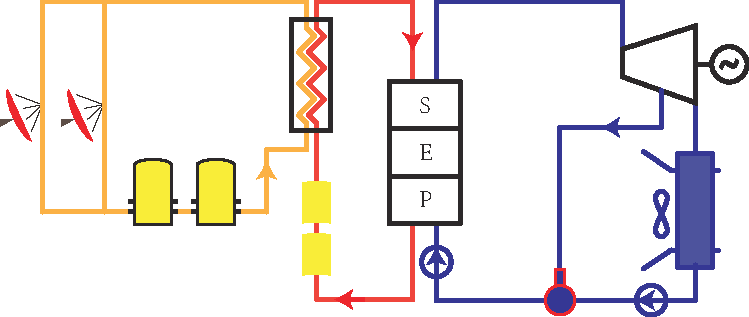
\includegraphics[width=0.7\textwidth]{fig/air-oil}
\caption{使用空气-导热油换热器的太阳能光热系统示意图}\label{fig:air-oil}
\end{figure}

\begin{figure}[htbp]
\centering
	\begin{subfigure}[b]{0.4\columnwidth}
	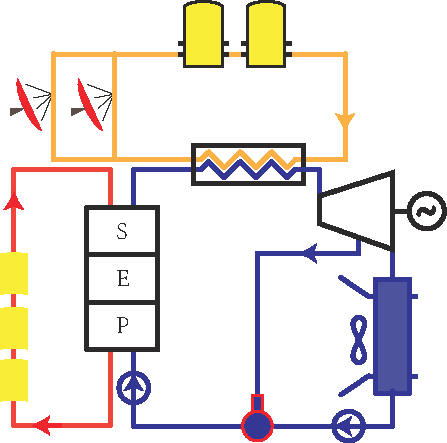
\includegraphics[width = \columnwidth]{fig/air-water1}
	\caption{}\label{fig:air-water_1}
	\end{subfigure}
	~
\begin{subfigure}[b]{0.4\columnwidth}
	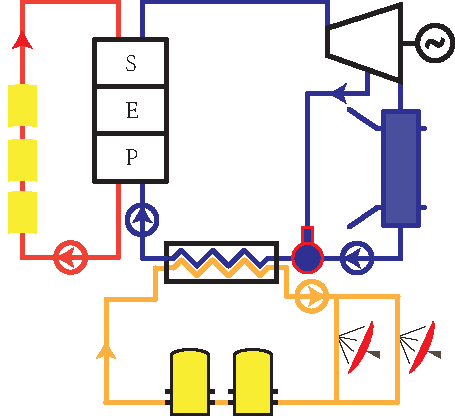
\includegraphics[width = \columnwidth]{fig/air-water2}
	\caption{}\label{fig:air-water_2}
	\end{subfigure}
	\caption{两种使用了空气-水换热器的梯级系统案例}
	\label{fig:air-water}
\end{figure}

第二种是在空气回路和水回路之间使用的空气-水换热器。图\ref{fig:air-water_1}和图\ref{fig:air-water_2}是使用了这种换热器的两个梯级系统方案。图\ref{fig:air-water_1}中,热空气在为斯特林机组供热后,再流经空气-水换热器,为水的过热过程提供热量。图\ref{fig:air-water_2}中,热空气在为斯特林机组供热后,再流经空气-水换热器,为水的预热过程提供热量。

在这种方案中,空气为水提供热量。图\ref{fig:air-water_c}中给出了两种使用空气-水换热器的太阳能梯级系统方案。其中,图\ref{fig:air-water_1_c}给出的是使用加热过斯特林机之后的热空气来继续为过热蒸汽提供热量的方案。这是可行的,因为热空气可以提升水的吸热过程的平均温度从而提高朗肯循环的效率。另一方面,在传统的太阳能槽式系统中,主蒸汽温度受到导热油极限温度的限制,这不利于提升朗肯循环的效率。在这个梯级系统中,朗肯循环的主蒸汽温度可以提高到高于400$\mathrm{^\circ C}$以消除导热油极限温度带来的负面影响。
这一系统方案将作为主要研究方案在接下来的内容里详细讨论。图\ref{fig:air-water_2_c}给出的是使用加热过斯特林机后的热空气预热给水的方案。由于斯特林机出口的空气温度较高,而朗肯循环的给水温度较低,二者之间存在很大的温差。如果采用此方案,则换热过程产生的㶲损很大。此外,由于给水温度的提升导致太阳能场内的导热油的平均温度也会有所上升,这将降低太阳能场的集热效率,进而降低整个系统的效率。

\subsection{循环之间热量利用的系统结构}
\label{sec:HRBC}

根据热力学第二定律,不可能从单一热源吸热使之完全转换为有用的功而不产生其他影响。对于热机,它同时需要热源和冷源来将热能转化为机械能。典型热机的热功转换图如图\ref{fig:engines}所示。在热力循环中,从热源吸收的热量,只有一部分可以通过热机转化为机械功,其它部分需要传递到冷源。卡诺定理从根本上限制了与热源温度和冷源温度有关的热功转换比,即$\dfrac{W}{Q_H} \leqslant \dfrac{T_H - T_C}{T_H}$,其中$T_H$和$T_C$的单位为$\mathrm{K}$。

\begin{figure}[ht]
\centering 
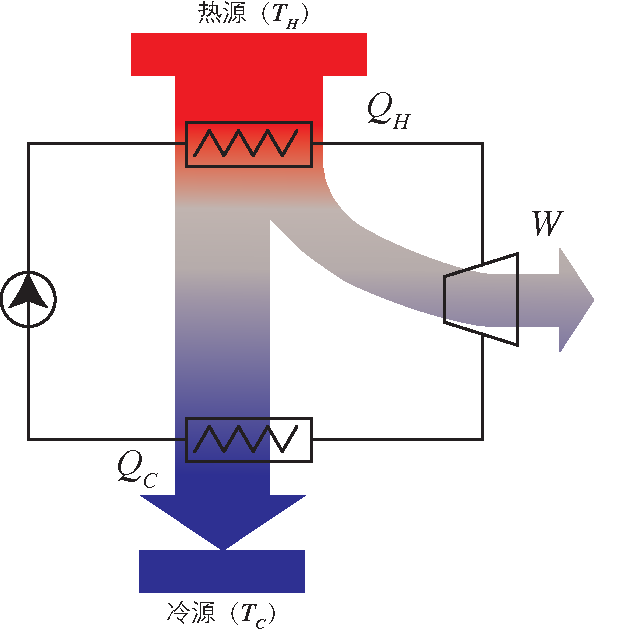
\includegraphics[width=0.5\textwidth]{fig/engines}
\caption{典型热机的热功转换图}
\label{fig:engines}
\end{figure}

不同的热机采用不同的热力循环来实现热功转换,它们有着不同的最佳工作温度。朗肯循环的最佳工作温度较低,斯特林循环的最佳工作温度较高。太阳能光热应用中斯特林循环和朗肯循环的$T$-$s$图如图\ref{fig:cycles}所示。

\begin{figure}[ht]
\centering 
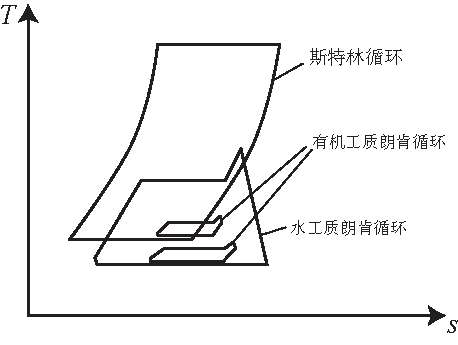
\includegraphics[width=0.5\textwidth]{fig/cycles}
\caption{太阳能光热应用中斯特林循环和朗肯循环热力循环的$T$-$s$图}\label{fig:cycles}
\end{figure}

由于每个热力循环都具有吸热和放热过程,因此可以组合多种热力循环,使一个循环(底部循环)吸收利用另一个循环(顶部循环)释放的热量,不同的循环可以耦合起来用于梯级发电。

\noindent \begin{figure}[htbp]
\centering
	\begin{subfigure}[b]{0.4\columnwidth}
	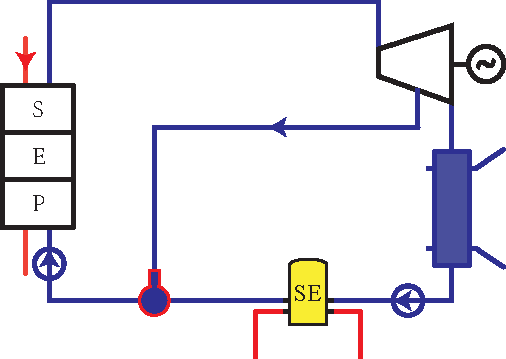
\includegraphics[width = \columnwidth]{fig/Stirling-Rankine}
	\caption{}\label{fig:Stirling-Rankine}
	\end{subfigure}
	~
\begin{subfigure}[b]{0.4\columnwidth}
	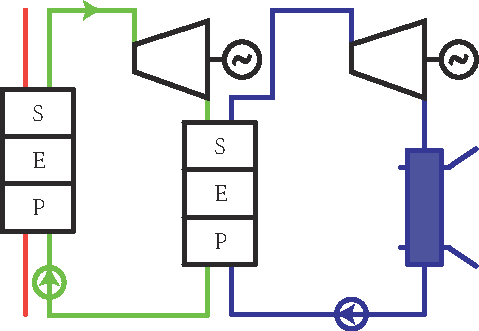
\includegraphics[width = \columnwidth]{fig/SeriesRankine}
	\caption{}\label{fig:Rankine-Rankine}
	\end{subfigure}
	\caption{采用多个热力循环之间热量回收利用的梯级系统结构图}
	\label{fig:coupledCycles}
\end{figure}

%In our basic systems (see Figure~\ref{fig:PTPD}), Rankine cycle and Stirling cycle can be coupled for cascade usage. 
%Figure~\ref{fig:coupledCycles} shows two configurations of the cascade systems with heat recovery between cycles. 
%For a traditional Stirling engine, to enhance the performance, cooling water is used to absorb the heat released by the engine. The absorbed heat is wasted without reuse.
%In Figure~\ref{fig:Stirling-Rankine}, condensate of the Rankine cycle is used to cool the Stirling engine. Rejected heat of the Stirling cycle can be recycled by Rankine cycle. 
%For organic Rankine cycles, different working fluids determine the working temperature zones. It is feasible to reuse the condensation heat of an organic Rankine cycle by another organic Rankine cycle.
%In Figure~\ref{fig:Rankine-Rankine}, two organic Rankine are coupled together for power generation. The bottoming cycle uses the condensation heat of the topping cycle for preheating, evaporation and superheating.
图\ref{fig:coupledCycles}给出了热力循环之间热量回收利用的梯级系统的两种系统结构。
传统的斯特林机为了提高性能,使用冷却水来吸收斯特林机释放的热量,吸收的热量往往被浪费掉而没有回收利用。
在图\ref{fig:Stirling-Rankine}中,采用朗肯循环的凝结液来冷却斯特林机。斯特林循环排出的热量可以通过朗肯循环回收利用。
对于有机朗肯循环,不同的工作流体决定循环的工作温度区间。用一个有机朗肯循环重复利用另一个有机朗肯循环的凝结热是可行的。在图\ref{fig:Rankine-Rankine}中,两个有机朗肯循环耦合在一起用于发电。底部循环利用顶部循环的凝结热来实现预热,蒸发和过热,再利用朗肯循环发电。

%%\section{System topology selection}
%\section{系统拓扑结构的选择}
%\label{sec:sts}
%%\subsection{Rankine cycle fluid}
%\subsection{朗肯循环工质}
%
%%There are two important aspects to consider when selecting the working fluid of the Rankine cycle solar power system:
%
%%\subsection{Solar chimney}
%\subsection{太阳能烟囱技术}
%
%%Section~\ref{sec:sc} shows the idea of coupling solar chimney to concentrated solar thermal power generation technologies.
%%However, the efficiency of current solar chimney system is very low. Primary design data of solar chimney power plants with different location, different chimney height and collector height are shown in Table~\ref{tab:sc}~. The preliminary design parameters are selected and determined for a nominal solar irradiation intensity of 1000$\,\mathrm{W/m^2}$ and the nominal plant power of 5$\,\mathrm{MW}$. From the table, it can be found that the chimney efficiency and total efficiency are very low and the technology is still in the developing stage.
%第\ref{sec:sc}小节提出了将太阳能烟囱组合到太阳能槽式光热发电技术的观点。
%然而,目前的太阳能烟囱系统的效率非常低。Bilgen和Rheault利用MATLAB建立了5$\,\mathrm{MW}$的太阳能烟囱模型\cite{Bilgen2005}。他们对不同地理位置,不同烟囱高度和集热器高度的太阳能烟囱电站进行了模拟分析。其主要设计数据及计算结果如表\ref{tab:sc}所示。 初步的设计参数为太阳辐射强度为1000$\,\mathrm{W/m^2}$,额定功率为5$\,\mathrm{MW}$。从表中可以发现,烟囱效率和系统总效率都很低,太阳能烟囱技术仍处于初步发展阶段。
%\begin{table}[htbp]
%\setlength{\abovecaptionskip}{-10pt}
%	\caption{太阳能烟囱设计参数及模拟结果}
%	\begin{center}
%	\begin{tabular}{ccccc}
%		\toprule
%		地理位置	&Ottawa    &Winnipeg    &Edmonton    &Schlaich\\
%		\midrule
%		集热棚直径 (m)    &	1110	&	1110	&	1110	&	1110 \\
%  集热棚面积 ($\mathrm{m^2}$)    & 950000    & 950000	&	950000	&	950000\\
%  烟囱高度 (m)    &123    &60    &    35&    547\\
%  集热器高度 (m)    &848    &975    &1024    &    -\\
%  烟囱直径 (m)    &54    &54    &54    &54\\
%  集热棚内温升 ($\mathrm{^\circ C}$)    &25.9    &25.9    &25.9    &25.9\\
%  气流速度 (m/s)&9.1    &9.1    &9.1    &9.1\\
%  总压头 (Pa)&518.3    &518.3    &518.3    &383.3\\
%  平均效率\\
%  集热棚 (\%)    &56.00    &56.00    &56.00    &56.24\\
%  烟囱 (\%)    &1.82    &1.82    &1.82    &1.45\\
%  涡轮机 (\%)    &77.0    &77.0    &77.0    &77.0\\
%  系统整体 (\%)    &0.79    &0.79    &0.79    &0.63\\
%		\bottomrule
%	\end{tabular}
%	\end{center}
%	\label{tab:sc}
%\end{table}
%
%%Besides, a solar chimney is costly and requires vast land, which is adverse to the future deployment of solar cascade demo system. With these considerations, the solar chimney plans are not adopted for the cascade system. 
%另外,太阳能烟囱成本高,占地面积大,不利于今后搭建太阳能光热梯级发电示范系统。鉴于这些,梯级系统不采用太阳能烟囱技术。
%
%%\subsection{Collector series connection}
%\subsection{集热器串联连接}
%\label{sec:seriesConnection}
%%Each type of collector has its own suitable temperature range. It is feasible to heat the HTF step by step using different types of collectors with series connection.
%每种类型的集热器都有其适宜的工作温度范围。使用串联的不同类型的集热器逐步加热传热流体是可行的。
%
%%A collector series connection is proposed in Section~\ref{sec:csc} (see Figure~\ref{fig:SeriesCollector}) depending on the basic systems. In this configuration, air is heated in the trough collectors and dish receivers consequently. After providing heat for the Stirling engines, the hot air flows into the heat exchanger to provide heat for the Rankine cycle. In this topology, air is used as the HTF for the solar trough, this idea is only numerically and experimentally studied,~\cite{Good2015,Good2016} no commercial applications can be found up to now. This technology is mainly constrained by the low conductivity and low heat capacity of air, which leads to low system efficiency. For this consideration, this topology is not adopted due to the air parabolic trough technology.
%本文根据基本系统(槽式-朗肯循环系统和碟式-斯特林机系统),在第\ref{sec:csc}节(见图\ref{fig:SeriesCollector})提出了一种集热器串联连接的方案。在这种方案中,空气依次在槽式集热器和碟式集热器中被加热。为斯特林机提供热量后,热空气流入换热器为朗肯循环提供热量。在这种拓扑结构中,空气被用作太阳能槽的传热流体,这个想法目前只有少数研究人员进行了数值和实验研究,至今还没有商业应用\cite{Good2015,Good2016}。这种技术最大的技术难题在于,空气导热系数低,热容量低,导致系统效率非常低。由于该拓扑结构使用了尚不成熟的空气槽式集热技术,故不采用这种方案。
%
%%It can be a good choice to apply flat plate solar collectors and parabolic trough collectors in traditional solar power tower plant that uses water as the HTF (such as Solar One). As demonstrated in Figure~\ref{fig:seriesCollection}, condensed water is heated by the flat plate solar collectors and feedwater is heated by the parabolic trough collectors. Flat plate collectors and parabolic trough collectors have much lower unit thermal cost compared to solar power tower. The addition of flat plate collectors and parabolic trough collectors can effectively reduce the cost of the system. Although this scheme is promising and deserves further research, the cascade system in this thesis will not consider it for the requirement of solar power tower is adverse to the deployment of cascade demo system.
%有的太阳能塔式电厂采用水作为传热流体(如Solar One电厂),这时可以利用平板式太阳能集热器和(或)槽式集热器作为低温段的集热器。系统结构图如图\ref{fig:seriesCollection}所示,冷凝水由平板式集热器加热,给水由槽式集热器加热。与太阳能塔式电厂相比,平板式集热器和槽式集热器收集低温热量的单位热成本要低很多。平板式集热器和槽式集热器的串联连接加入可以有效降低系统发电成本。虽然该方案有很好的前景,值得进一步研究,但本文的梯级系统不考虑采用太阳能塔式系统,所以该方案留给后续研究工作。
%
%\begin{figure}[!ht]
%\centering 
%\includegraphics[width=0.5\textwidth]{fig/SeriesCollection}
%\caption{采用多种型式集热器串联连接的太阳能塔式发电系统}\label{fig:seriesCollection}
%\end{figure}
%
%%\subsection{Direct steam generation}
%\subsection{直接生产蒸汽技术}
%%Direct steam generation for solar thermal power generation has the advantages of having fewer components and no temperature drop due to an intermediate transfer. Besides, it is clear that water is characterized by lower environmental risk than thermal oil so that leakages in a DSG power plant do not represent an environmental hazard~\cite{Fernandez2010}. Water has a lower freezing temperature than thermal oil and solar salt: the efforts required to ensure adequate anti-freezing protection are significantly reduced. Water is also less corrosive than solar salt~\cite{Giglio2017}.
%在太阳能光热发电系统中应用直接生产蒸汽技术具有减少系统部件,不存在传热温差等优点。水具有比合成油和熔融盐更低的凝固点,不需要像其他传热流体一样做大量的防冻保护措施。水的腐蚀性也比合成油和熔融盐小\cite{Giglio2017}。此外,水对环境的污染风险要远低于其它传热流体,DSG电厂的泄漏不会对环境造成太大的破坏\cite{Fernandez2010}。
%
%%However, all the CSP commercial plants already built apply indirect steam generation, with the exception of the 5$\,\mathrm{MWe}$ DSG Thai Solar One (TSE-1) plant in Thailand (Thailand, 2012)~\cite{Khenissi2015}. 
%%The reason for this universally accepted choice must be found in the difficulties related to the flow control and manufacturing of equipment to be used in the presence of a two-phase flow in the absorber tubes. 
%%The behavior of the two-phase flow inside the absorber tubes of a parabolic-trough collector forces the implementation of a complex and expensive control system and the use of fast water streams in order to avoid stratified flow.
%然而,除了在泰国的装机容量为5$\,\mathrm{MWe}$的泰国太阳能一号(TSE-1)电厂(泰国,2012)外,所有已建成的CSP商业电厂都应用间接蒸汽发电\cite{Khenissi2015}。DSG方案没有被普遍接受的原因在于,吸热管中两相流区域的流量控制和制造工艺非常困难。槽式集热器的吸热管内存在两相流,需要配备复杂而昂贵的控制系统,并需要较快的流速以避免出现层流。
%
%%Besides, the receiver should be designed with care to ensure that the flux in the regions of vapor is less than the regions where boiling is taking place.
%%This is because the liquid's heat transfer coefficient is significantly higher than superheated steam. For similar solar flux values, burnout of the receiver may occur in the region where vapor exists on the other side of the receiver wall. 
%%Many concentrating collector designs require the receiver to change its attitude while tracking the sun. This change of attitude increases the possibility of high flux in the steam-containing receiver section.
%此外,应当谨慎设计接收器,以确保蒸汽区域的光通量小于发生沸腾的区域。这是因为液体的传热系数明显高于过热蒸汽。如果二者光通量接近,则接收器存在蒸汽的区域则可能因不能快速带走热量而出现灼伤。
%还有许多集热器的跟踪系统要求接收器在跟踪太阳时改变其方位。这种方位的调整增大了含蒸汽的接收器部分接受到高光通量的可能性。
%%Two examples of solar Rankine power systems where the engine working fluid vapor is generated directly in the receiver are the Solar One Pilot Plant at Barstow, CA and the solar organic Rankine cycle module built by Ford Aerospace and Communications Corporation. Because Solar One is a central receiver system, the vertical-tube receiver remains stationary and liquid level control is relatively easy. The vertical tubes of the receiver are made of a material with a high melting point and thus can withstand high temperatures in the upper regions where vapor is being superheated. Tube burnout is avoided in the Ford Aerospace receiver design because the inner wall of the \rule{•‹width›}{•‹height›}eceiver is a copper shell with tubes wound around its exterior. The high thermal conductivity of the copper shell provides an averaging effect on receiver temperature, and superheat is attained without burnout of the receiver walls.
%			
%%Another problem related to DSG is the high value of the steam pressure inside the receiver tubes that must match the turbine inlet pressure. 
%%Indeed, handling of movable and flexible parts forming the collector's receiver tube at high pressure values is one of the major problems that the DSG technology faces at its early stages.
%与DSG相关的另一个问题是为了与汽轮机入口压力相匹配,接收器管内的蒸汽压力比较高。事实上,在高压下处理形成接收器吸热管的可移动和柔性部件是DSG技术面临的主要问题之一。
%
%%Applying direct steam generation may be a better choice in the cascade system in the future, however, it is not adopted for the cascade system for its immaturity.
%在未来的梯级系统中应用直接生产蒸汽技术可能是一个较好的选择。然而,由于其技术尚不成熟,现阶段梯级系统的技术方案不采用直接生产蒸汽技术。
%
%%\subsection{Heat exchanger between circuits}
%\subsection{回路间的换热}
%
%%Section~\ref{sec:hebc} introduces two types of heat exchangers that may be applied in the solar thermal cascade system -- the air-oil heat exchanger (see in Figure~\ref{fig:air-oil_c}) and the air-water heat exchanger (see in Figure~\ref{fig:air-water_c}). 
%第\ref{sec:hebc}节介绍了两种可应用于太阳能梯级集热系统的换热器,空气-导热油交换器(参见图\ref{fig:air-oil_c})和空气-水换热器(参见图\ref{fig:air-water_c})。
%
%\begin{figure}[ht]
%\centering 
%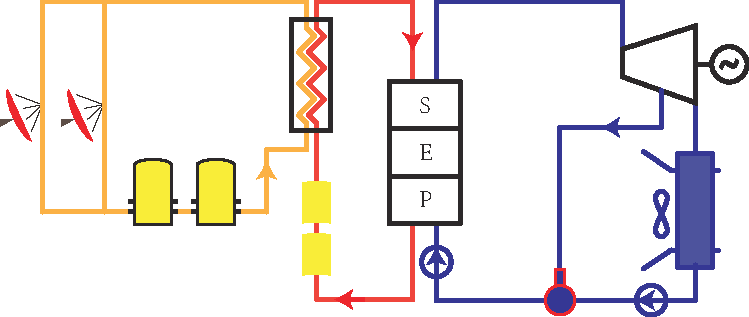
\includegraphics[width=0.7\textwidth]{fig/air-oil}
%\caption{使用空气-导热油换热器的太阳能光热系统示意图}\label{fig:air-oil_c}
%\end{figure}
%
%\noindent \begin{figure}[htbp]
%\centering
%	\begin{subfigure}[b]{0.4\columnwidth}
%	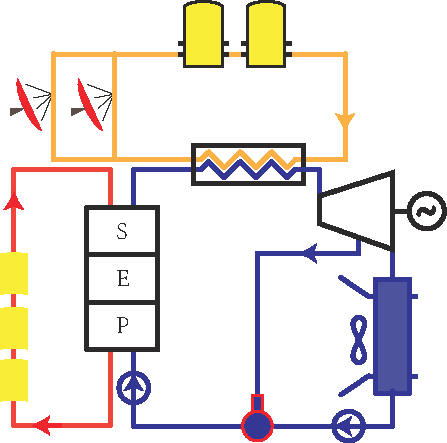
\includegraphics[width = \columnwidth]{fig/air-water1}
%	\caption{}\label{fig:air-water_1_c}
%	\end{subfigure}
%	~
%\begin{subfigure}[b]{0.4\columnwidth}
%	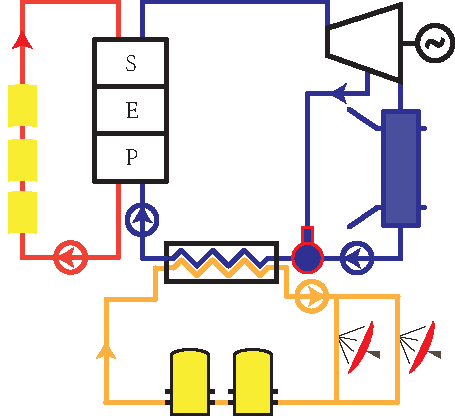
\includegraphics[width = \columnwidth]{fig/air-water2}
%	\caption{}\label{fig:air-water_2_c}
%	\end{subfigure}
%	\caption{两种使用了空气-水换热器的梯级系统案例}
%	\label{fig:air-water_c}
%\end{figure}
%
%%For the first type, air provides heat for oil. It is not economic for several reasons. First, The temperature of the heat transfer oil can not be further increased. The temperature of the oil is not limited by the parabolic trough collectors. The temperature of the oil is constrained by the oil properties and heat collecting temperature of the trough collectors can exceed this value. In high temperature conditions, oil may deterioration, evaporation, decompose, which has a negative impact on the stable and safe operation of the system. Second, using dish to provide heat for the oil is not suitable since the dish is designed for higher temperature collections and it's less cost-effective compared with parabolic trough.
%对于第一种类型,空气为导热油提供热量。从几个方面来看,这是不经济的。首先,此方案并不能进一步提高导热油的温度。导热油的极限温度受到本身物质属性的限制,而并非受限于槽式集热器,槽式集热器的集热温度可以超过这个值。在高温条件下,油品可能会变质,蒸发,分解,对系统的安全稳定运行产生不利影响。其次,使用碟式集热器为导热油提供热量是不经济的,因为碟式集热器是为了收集更高温度的热量而设计的,与槽式集热器相比,它在收集中低温热量时效益更低。
%
%%For the second type, air provides heat for water. Two kinds of solar systems using air-water heat exchanger can be found in Figure~\ref{fig:air-water_c}. Figure~\ref{fig:air-water_1_c} shows the scheme that air after the Stirling engine is used to overheat the steam. It's feasible since the air can increase the average temperature of the endothermic process of the water to increase the efficiency of Rankine cycle. On the other hand, in a conventional solar trough system, the main steam temperature is limited by the oil, which is not conductive to Rankine cycle efficiency. In this proposed cascade system, the main steam temperature of the Rankine cycle can be raised to be higher than 400$\mathrm{^\circ C}$ to eliminate the negative effect of the oil.
%%This is the scheme that will be discussed in detail in the next few chapters. Figure~\ref{fig:air-water_2_c} shows the scheme that air after the Stirling engine is used to preheat the feed water. It is not a good choice since the temperature difference of the heat transfer process is large and it provides no benefits to increase the inlet temperature of the steam turbine.
%对于第二种类型,空气为水提供热量。图\ref{fig:air-water_c}中给出了两种使用空气-水换热器的太阳能梯级系统方案。其中,图\ref{fig:air-water_1_c}给出的是使用加热过斯特林机之后的热空气来继续为过热蒸汽提供热量的方案。这是可行的,因为热空气可以提升水的吸热过程的平均温度从而提高朗肯循环的效率。另一方面,在传统的太阳能槽式系统中,主蒸汽温度受到导热油极限温度的限制,这不利于提升朗肯循环的效率。在这个梯级系统中,朗肯循环的主蒸汽温度可以提高到高于400$\mathrm{^\circ C}$以消除导热油极限温度带来的负面影响。
%这一系统方案将作为主要研究方案在接下来的内容里详细讨论。图\ref{fig:air-water_2_c}给出的是使用加热过斯特林机后的热空气预热给水的方案。由于斯特林机出口的空气温度较高,而朗肯循环的给水温度较低,二者之间存在很大的温差。如果采用此方案,则换热过程产生的㶲损很大。此外,由于给水温度的提升导致太阳能场内的导热油的平均温度也会有所上升,这将降低太阳能场的集热效率,进而降低整个系统的效率。
% 
%%\subsection{Heat recovery between cycles}
%\subsection{循环之间热量利用}
%%As it is mentioned in Section~\ref{sec:HRBC}, different thermodynamic cycles work at different optimum working temperatures. Since each thermodynamic cycle has endothermic and exothermic processes, a bottoming cycle may use the released heat of a topping cycle.
%正如在第\ref{sec:HRBC}节中提到的,不同的热力循环有着在不同的最佳工作温度。由于每个热力循环都具有吸热和放热过程,因此可以组合多种热力循环,使一个循环(底部循环)吸收利用另一个循环(顶部循环)释放的热量。在我们的基本系统中(参见图\ref{fig:PTPD}),朗肯循环和斯特林循环可以耦合起来用于梯级发电。
%
%\noindent \begin{figure}[htbp]
%\centering
%	\begin{subfigure}[b]{0.4\columnwidth}
%	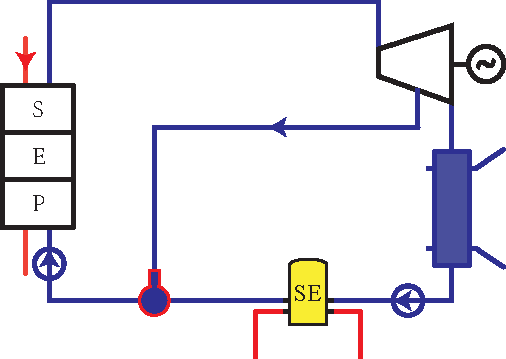
\includegraphics[width = \columnwidth]{fig/Stirling-Rankine}
%	\caption{}\label{fig:Stirling-Rankine}
%	\end{subfigure}
%	~
%\begin{subfigure}[b]{0.4\columnwidth}
%	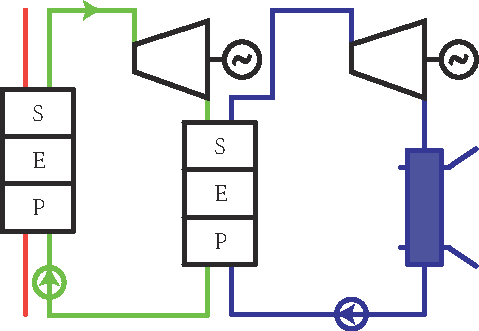
\includegraphics[width = \columnwidth]{fig/SeriesRankine}
%	\caption{}\label{fig:Rankine-Rankine}
%	\end{subfigure}
%	\caption{采用多个热力循环之间热量回收利用的梯级系统结构图}
%	\label{fig:coupledCycles}
%\end{figure}
%
%%In our basic systems (see Figure~\ref{fig:PTPD}), Rankine cycle and Stirling cycle can be coupled for cascade usage. 
%%Figure~\ref{fig:coupledCycles} shows two configurations of the cascade systems with heat recovery between cycles. 
%%For a traditional Stirling engine, to enhance the performance, cooling water is used to absorb the heat released by the engine. The absorbed heat is wasted without reuse.
%%In Figure~\ref{fig:Stirling-Rankine}, condensate of the Rankine cycle is used to cool the Stirling engine. Rejected heat of the Stirling cycle can be recycled by Rankine cycle. 
%%For organic Rankine cycles, different working fluids determine the working temperature zones. It is feasible to reuse the condensation heat of an organic Rankine cycle by another organic Rankine cycle.
%%In Figure~\ref{fig:Rankine-Rankine}, two organic Rankine are coupled together for power generation. The bottoming cycle uses the condensation heat of the topping cycle for preheating, evaporation and superheating.
%图\ref{fig:coupledCycles}给出了热力循环之间热量回收利用的梯级系统的两种系统结构。
%传统的斯特林机为了提高性能,使用冷却水来吸收斯特林机释放的热量,吸收的热量往往被浪费掉而没有回收利用。
%在图\ref{fig:Stirling-Rankine}中,采用朗肯循环的凝结液来冷却斯特林机。斯特林循环排出的热量可以通过朗肯循环回收利用。
%对于有机朗肯循环,不同的工作流体决定循环的工作温度区间。用一个有机朗肯循环重复利用另一个有机朗肯循环的凝结热是可行的。在图\ref{fig:Rankine-Rankine}中,两个有机朗肯循环耦合在一起用于发电。底部循环利用顶部循环的凝结热来实现预热,蒸发和过热,再利用朗肯循环发电。

%\section{Selected system topology}
\section{选定的梯级系统拓扑结构}
\label{sec:sst}
%Considered all the conditions in Section~\ref{sec:std} and Section~\ref{sec:sts}, two system topologies are chosen for this research as shown in Figure~\ref{fig:CascadeSystems}. 
考虑了第\ref{sec:std}节和第\ref{sec:sts}节中的所有因素,本文选择了两个系统拓扑结构进行太阳能光热梯级发电技术的研究,其系统结构图如图\ref{fig:CascadeSystems}所示。

%第二种方案需要考虑是否用两个空气换热器
\noindent \begin{figure}[htbp]
\centering
	\begin{subfigure}[b]{0.4\columnwidth}
	\includegraphics[width = \columnwidth]{fig/CascadeSystem1}
	\caption{}\label{fig:CascadeSystem1}
	\end{subfigure}
	~
\begin{subfigure}[b]{0.4\columnwidth}
	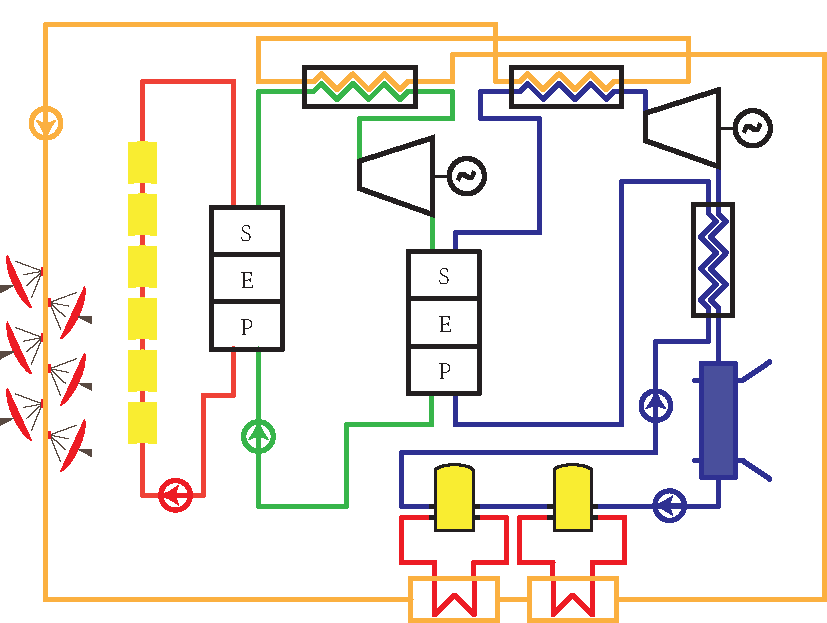
\includegraphics[width = \columnwidth]{fig/CascadeSystem2}
	\caption{}\label{fig:CascadeSystem2}
	\end{subfigure}
	\caption{两种选定的梯级系统拓扑结构图}
	\label{fig:CascadeSystems}
\end{figure}

%In Figure~\ref{fig:CascadeSystem1}, the cascade system has the following features:
图\ref{fig:CascadeSystem1}中的梯级系统具有以下特点:
\begin{itemize}
%  \item \emph{Multiple types of collectors.} Trough collectors are applied for lower temperature heat collection and dish collectors are applied for higher temperature heat collection. This helps to reduce the cost and improve the efficiency.
  \item \emph{选用了多种型式的集热器。}槽式集热器用于较低温度的集热,碟式集热器用于较高温度的集热。这有助于降低成本并提高系统效率。
%  \item \emph{Multiple types of thermodynamic cycles.} Rankine cycle is applied for lower temperature heat utilization. Stirling cycle is applied for higher temperature heat utilization.
  \item \emph{使用了多个热力循环。}朗肯循环适用于较低温度的热利用。斯特林循环适用于更高温度的热利用。二者工作区间的不同使得底部循环利用顶部循环释放的热量成为可能。
%  \item \emph{Air-water heat exchanger.} An extra air-water heat exchanger is applied to increase the temperature of the main steam, which helps to improve the efficiency of Rankine cycle. On the other hand, it can overcome the disadvantage of low limit temperature of heat transfer oil in conventional solar trough systems, which helps to achieve higher main steam parameters than traditional solar trough systems. 
  \item \emph{使用了空气-水换热器。} 使用空气-水换热器来提高主蒸汽的温度,这有助于提高朗肯循环的效率。 另一方面它克服了传统太阳能槽式系统中导热油极限温度较低的缺点,有助于实现比传统太阳能槽式系统更高的主蒸汽参数,进而提升朗肯循环的效率。 
%  \item \emph{Condensate for Stirling engine cooling.} Condensate of the Rankine cycle is used to cool the Stirling engine. Rejected heat of the Stirling cycle can be reused by Rankine cycle, which helps to improve the overall system efficiency.
  \item \emph{采用朗肯循环的凝结液来冷却斯特林机。} 采用朗肯循环的凝结液来冷却斯特林机。斯特林循环的废弃热量可以通过朗肯循环回收利用,这有助于提高系统的整体效率。
\end{itemize}

%In Figure~\ref{fig:CascadeSystem2}, the cascade system also has the features mentioned above. Besides, it uses different kinds of organic fluid as the working fluid, which adapts more general working temperature for solar energy systems. Figure~\ref{fig:Ex_CascadeSystem2} shows a calculation example of the cascade system.

图\ref{fig:CascadeSystem2}中的梯级系统也具有上述特点。此外,它采用不同种类的有机工质作为工作流体,使太阳能光热系统具有更广泛的工作温度区间,可以适用于多种能量需求。它的一个计算案例如图\ref{fig:Ex_CascadeSystem2}所示。
\begin{figure}[htbp]
\centering 
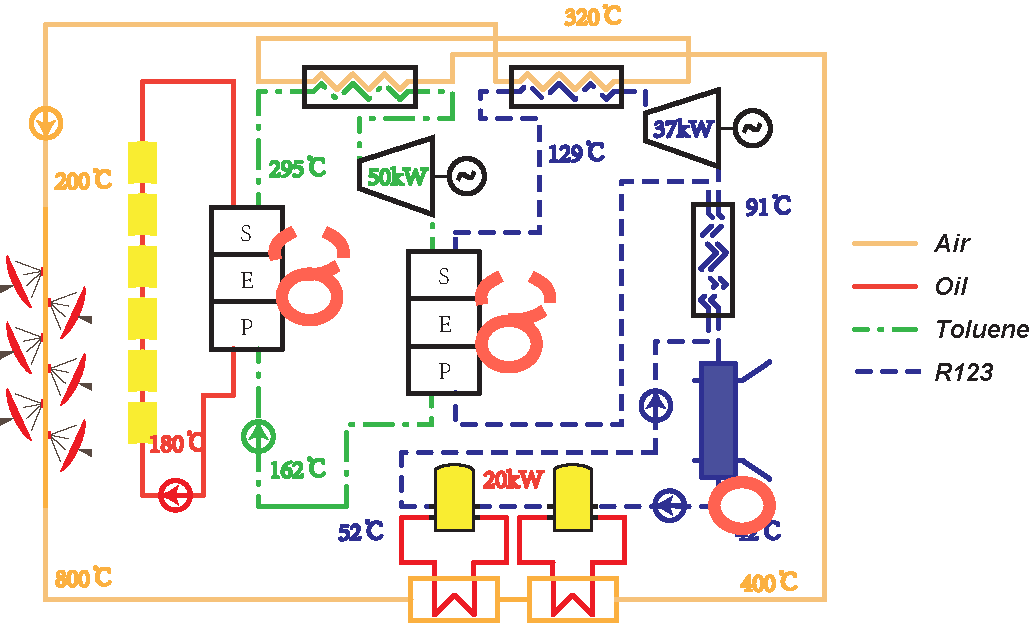
\includegraphics[width=0.7\textwidth]{fig/Ex_CascadeSystem2}
\caption{采用多级朗肯循环的一个计算案例}
\label{fig:Ex_CascadeSystem2}
\end{figure}
%Both cascade systems will be modeled for investigation. However, considering the more extensive application of steam Rankine cycle, the system described in Figure~\ref{fig:CascadeSystem1} will be used as the main research content in the following chapters.
本文将重点分析这两个梯级系统。但是,考虑到蒸汽朗肯循环的应用更加广泛,以及图\ref{fig:CascadeSystem1}所描述的系统还考虑了斯特林循环,研究领域更加广阔,
下面的章节将使用该系统作为主要研究内容。

%\section{Conclusion}
\newpage
\section{本章小结}
%This chapter systematically introduces a number of considerations in cascade solar thermal system design. These considerations include Rankine cycle fluid type, solar chimney, collector series connection, direct steam generation, heat exchanger between circuits and heat recovery between cycles. 
本章系统地研究了太阳能光热梯级发电的拓扑结构。考虑了。
%These considerations are carefully checked for the cascade system study. Combining with the research direction, two typical system topologies suitable for the deployment of cascade demo system are put forward. These two typical system topologies have the following features:
接着,本文结合梯级系统的研究内容,并考虑到梯级示范系统的建设工作,针对各因素进行了详细分析,提出了两种适用于太阳能光热梯级发电的典型的系统拓扑结构。这两种典型的系统拓扑具有以下特点:

\begin{itemize}
%  \item Multiple types of collectors are applied.
  \item 使用了多种型式的集热器。
%  \item Multiple kinds of thermodynamic cycles are applied. 
  \item 使用了多个热力循环。
%  \item Air-water heat exchanger is applied to increase the Rankine cycle efficiency.
  \item 使用了空气-水换热器来提高朗肯循环的效率。
%  \item Condensate for Stirling engine cooling to recover the heat rejected by the engine.
  \item 使用朗肯循环的凝结液来冷却斯特林机。
\end{itemize}

%It is worthy noting that some of the considerations of the system topology design deserves more concern in the future. For example, a solar power tower combined with parabolic trough collectors and flat plates as shown in Figure~\ref{fig:seriesCollection} effectively utilizes the characteristics of the collectors. Besides, when the technology of direct steam generation is mature, it is worthy to apply it in cascade system for its less equipment required and no temperature loss feature.
值得注意的是,系统拓扑设计的一些考虑因素有待后续研究工作进行研究。 例如,塔式太阳能发电技术与槽式集热器和平板式集热器的组合,如图\ref{fig:seriesCollection}所示,该系统结构有效地利用了各种集热器的工作特性,有利于提升系统的效率并降低系统成本。另外,当直接生产蒸汽技术成熟时,考虑到其具有所需设备少,不存在温度损失的特点,值得将其应用于太阳能光热梯级发电系统。